% ============================================
% Chapitre 2 : Architecture Réseau
% ============================================
\chapter{Architecture Réseau}
\label{chap:architecture}

\section{Vue d'Ensemble}

L'architecture réseau déployée sur AWS repose sur un Virtual Private Cloud (VPC) configuré pour héberger l'ensemble de l'infrastructure de monitoring. Cette architecture a été conçue en tenant compte des limitations du Learner Lab AWS Academy.

\section{Schéma d'Architecture}

\begin{figure}[H]
\centering
\begin{tikzpicture}[
    node distance=1.5cm,
    box/.style={rectangle, draw=bluecustom, line width=1.5pt, minimum width=3cm, minimum height=1.2cm, align=center, font=\small},
    cloud/.style={rectangle, draw=awsorange, line width=2pt, minimum width=12cm, minimum height=8cm, align=center, rounded corners},
    subnet/.style={rectangle, draw=codegreen, line width=1pt, minimum width=11cm, minimum height=5.5cm, align=center, dashed}
]

% VPC
\node[cloud, label={[font=\bfseries]above:AWS VPC (10.0.0.0/16)}] (vpc) {};

% Subnet
\node[subnet, label={[font=\small]above:Subnet Public (10.0.1.0/24)}] at (0,-0.5) (subnet) {};

% Instances
\node[box, fill=awsorange!20] at (-4,-0.5) (zabbix) {Zabbix Server\\t3.large\\10.0.1.x};
\node[box, fill=codegreen!20] at (0,-0.5) (linux) {Client Linux\\t3.medium\\10.0.1.x};
\node[box, fill=codeblue!20] at (4,-0.5) (windows) {Client Windows\\t3.large\\10.0.1.x};

% Internet Gateway
\node[box, fill=awsorange!40] at (0,-4.5) (igw) {Internet Gateway};

% Internet
\node[box, fill=gray!20] at (0,-6.5) (internet) {Internet};

% Connections
\draw[->, thick] (igw) -- (internet);
\draw[->, thick] (subnet.south) -- (igw);

\end{tikzpicture}
\caption{Architecture réseau du projet AWS Zabbix}
\label{fig:architecture}
\end{figure}

\section{Création du VPC}

\subsection{Configuration du VPC}

Le VPC a été créé avec les paramètres suivants :

\begin{table}[H]
\centering
\caption{Configuration du VPC}
\label{tab:vpc-config}
\begin{tabular}{|l|l|}
\hline
\textbf{Paramètre} & \textbf{Valeur} \\
\hline
Nom & ELBadry-Zabbix-VPC \\
\hline
IPv4 CIDR & 10.0.0.0/16 \\
\hline
IPv6 & Désactivé \\
\hline
Tenancy & Default \\
\hline
\end{tabular}
\end{table}

\begin{figure}[H]
\centering
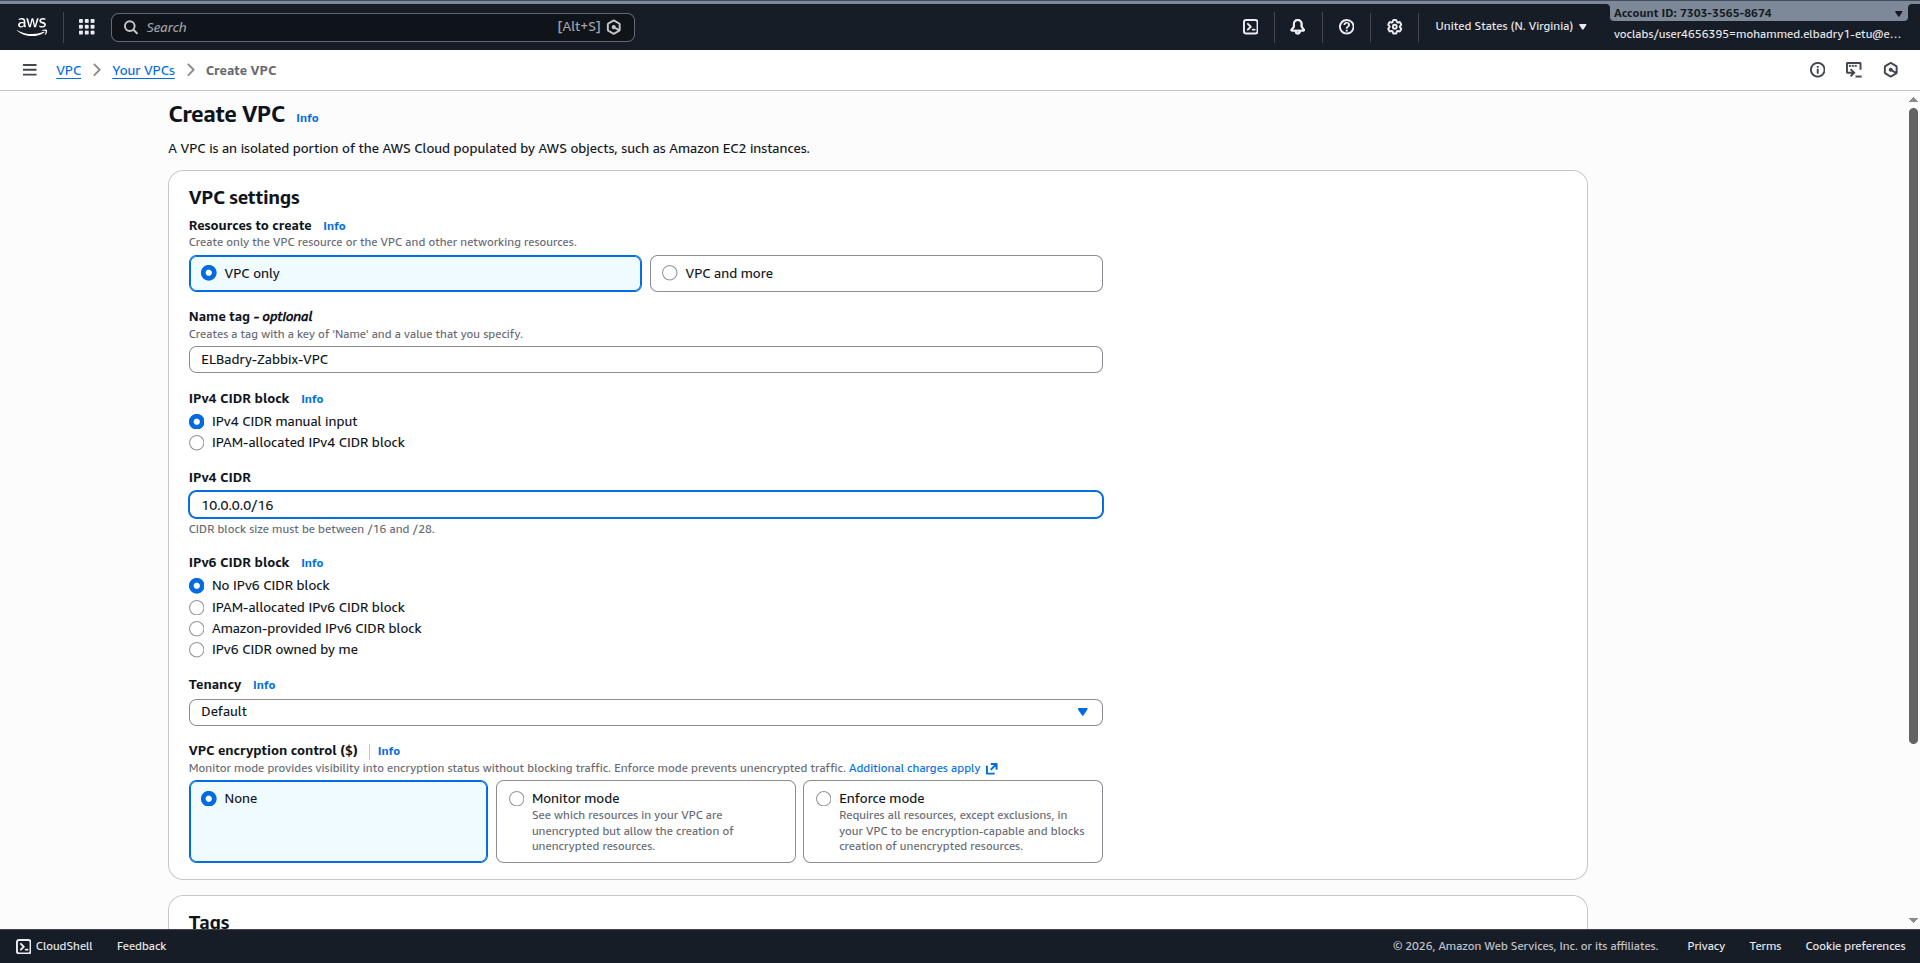
\includegraphics[width=0.9\textwidth]{images/01-vpc-creation.png}
\caption{Création du VPC dans la console AWS}
\label{fig:vpc-creation}
\end{figure}

\section{Configuration du Subnet}

\subsection{Subnet Public}

Un sous-réseau public a été créé pour héberger toutes les instances :

\begin{table}[H]
\centering
\caption{Configuration du Subnet}
\label{tab:subnet-config}
\begin{tabular}{|l|l|}
\hline
\textbf{Paramètre} & \textbf{Valeur} \\
\hline
Nom & ELBadry-Public-Subnet \\
\hline
VPC & ELBadry-Zabbix-VPC \\
\hline
Availability Zone & us-east-1a \\
\hline
IPv4 CIDR & 10.0.1.0/24 \\
\hline
Auto-assign Public IP & Activé \\
\hline
\end{tabular}
\end{table}

\begin{figure}[H]
\centering
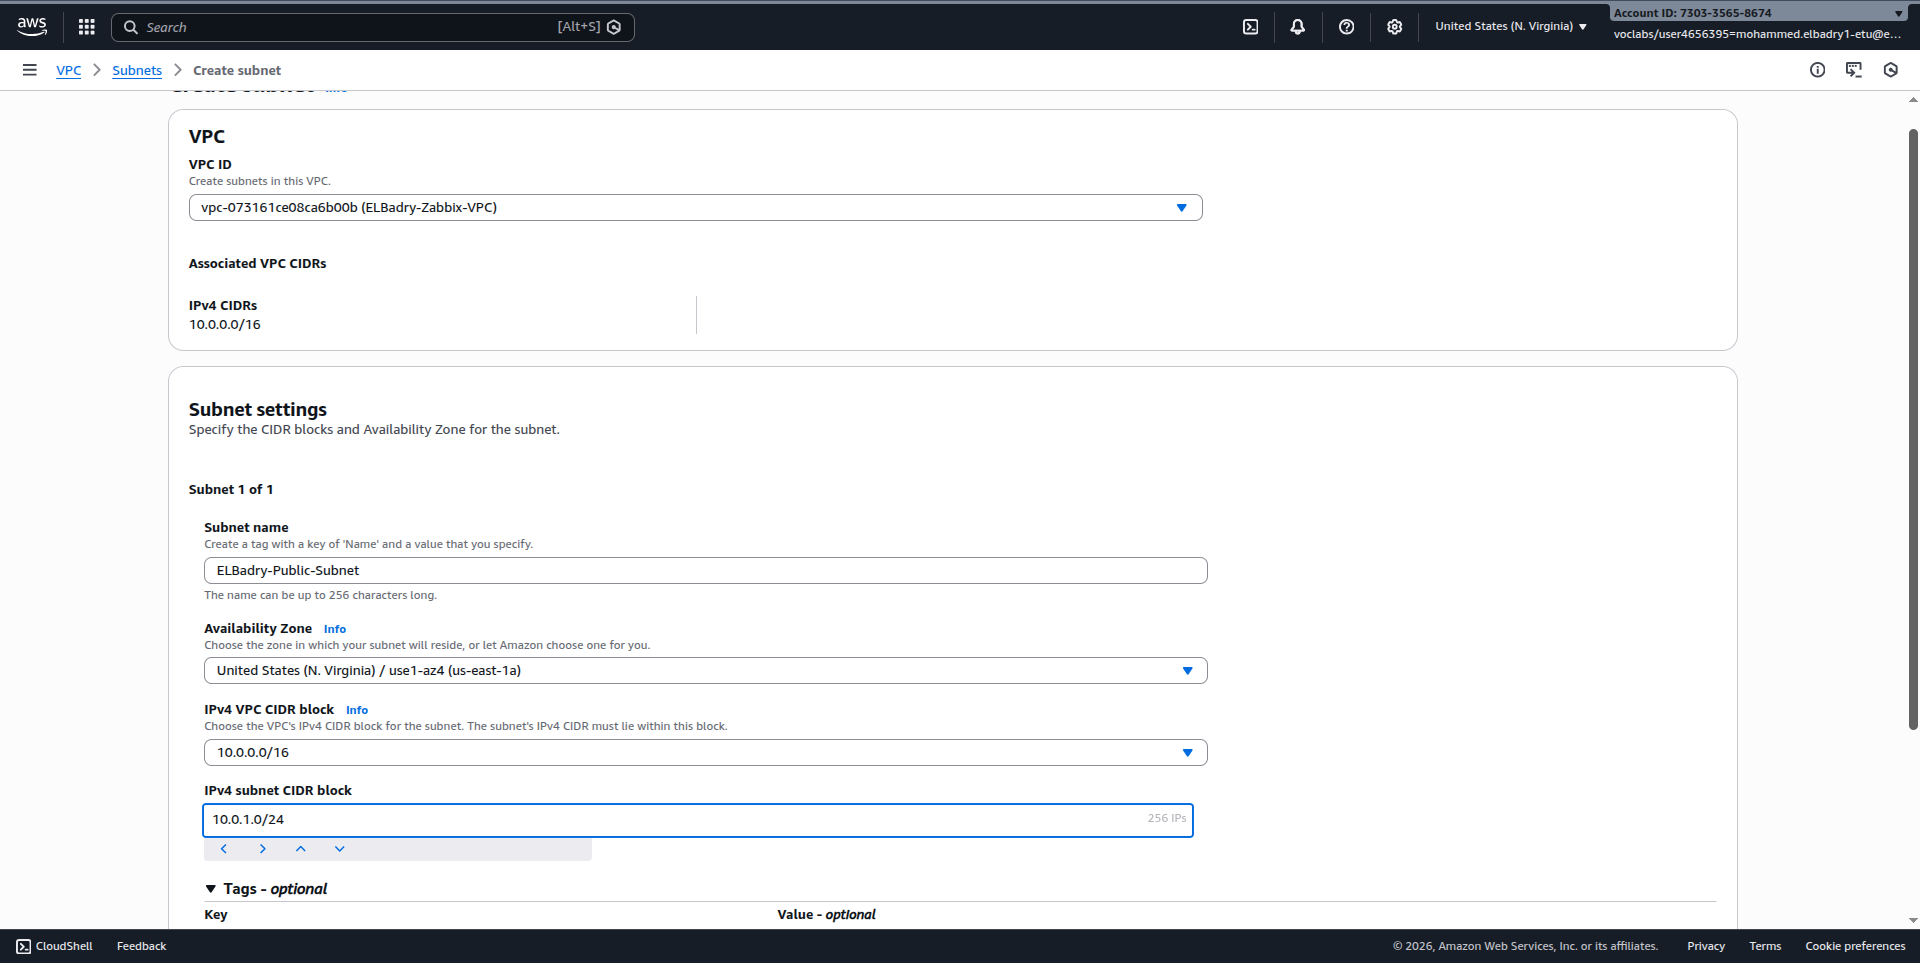
\includegraphics[width=0.9\textwidth]{images/02-subnet-configuration.png}
\caption{Configuration du Subnet public}
\label{fig:subnet-config}
\end{figure}

\section{Internet Gateway}

L'Internet Gateway permet aux instances du VPC de communiquer avec Internet :

\begin{enumerate}
    \item Création de l'Internet Gateway : \texttt{ELBadry-IGW}
    \item Attachement au VPC \texttt{ELBadry-Zabbix-VPC}
    \item Configuration de la table de routage avec la route \texttt{0.0.0.0/0} vers l'IGW
\end{enumerate}

\section{Security Groups}

\subsection{Security Group - Serveur Zabbix}

\begin{table}[H]
\centering
\caption{Règles du Security Group Zabbix Server}
\label{tab:sg-zabbix}
\begin{tabular}{|l|l|l|l|}
\hline
\textbf{Type} & \textbf{Port} & \textbf{Source} & \textbf{Description} \\
\hline
SSH & 22 & Mon IP & Accès SSH \\
\hline
HTTP & 80 & 0.0.0.0/0 & Interface Web Zabbix \\
\hline
HTTPS & 443 & 0.0.0.0/0 & Interface Web sécurisée \\
\hline
Custom TCP & 10050 & 10.0.0.0/16 & Zabbix Agent \\
\hline
Custom TCP & 10051 & 10.0.0.0/16 & Zabbix Trapper \\
\hline
\end{tabular}
\end{table}

\subsection{Security Group - Clients}

\begin{table}[H]
\centering
\caption{Règles du Security Group Clients}
\label{tab:sg-clients}
\begin{tabular}{|l|l|l|l|}
\hline
\textbf{Type} & \textbf{Port} & \textbf{Source} & \textbf{Description} \\
\hline
SSH & 22 & Mon IP & Accès SSH (Linux) \\
\hline
RDP & 3389 & Mon IP & Bureau à distance (Windows) \\
\hline
Custom TCP & 10050 & SG Zabbix Server & Agent Zabbix \\
\hline
\end{tabular}
\end{table}

\section{Tableau Récapitulatif des Ports}

\begin{table}[H]
\centering
\caption{Ports utilisés dans l'infrastructure}
\label{tab:ports}
\begin{tabular}{|l|l|p{7cm}|}
\hline
\textbf{Port} & \textbf{Service} & \textbf{Description} \\
\hline
22 & SSH & Accès sécurisé aux machines Linux \\
\hline
80 & HTTP & Interface Web Zabbix \\
\hline
443 & HTTPS & Interface Web Zabbix (sécurisé) \\
\hline
3389 & RDP & Bureau à distance Windows \\
\hline
10050 & Zabbix Agent & Communication passive (serveur → agent) \\
\hline
10051 & Zabbix Trapper & Communication active (agent → serveur) \\
\hline
\end{tabular}
\end{table}
